%-------------------------
%clang
%(c) H.Buchmann FHNW 2008
%export TEXINPUTS=.:${HOME}/fhnw/edu/:${HOME}/fhnw/edu/tinL/config/latex:${HOME}/fhnw/edu/config//:
%-------------------------
\documentclass{beamer}
\usepackage{beamer}
%---------------------
%local defines
%(c) H.Buchmann FHNW 2009
%$Id$
%---------------------
\newcommand{\target} {\beaglebone\xspace}
\newcommand{\targetS}{{\bf BBG}\xspace}
\newcommand{\host}   {{\em Host}\xspace}
\newcommand{\targetroot} {{\bf target-root}\xspace}
\newcommand{\kernel} {{\bf kernel}\xspace}
\renewcommand{\c}{{\bf C}\xspace}
\newcommand{\cpp}{{\bf C++}\xspace}
\newcommand{\posix}{{\bf POSIX}\xspace}


\usepackage[absolute]{textpos}
\setlength{\TPHorizModule}{1mm}
\setlength{\TPVertModule}{1mm}

\begin{document}

\title[Build]{Ein ganzes \linux}

\frame{\titlepage}

\begin{frame}{Um was geht es ?}
 \begin{itemize}
  \item ein \linux von Grund auf bauen
  \begin{itemize}
   \item nicht mehr so schwer wie auch schon
  \end{itemize}
  \item ein kleines angepasstes \linux
  \begin{itemize}
   \item grosse \linux gibt es schon
  \end{itemize}
  \item nicht v�llig automatisiert
  \item Alternative zu {\bf yocto} (\url{www.yoctoproject.org}) \& Co. 
 \end{itemize}
\end{frame}

\begin{frame}{Ziel}{\linux auf dem \target}
\begin{itemize}
 \item command based
 \item Ethernet/Wi-Fi
 \item \cod{ssh} 
 \item \cod{sshfs}
 \item moderne Toolchain inkl. {\em c++14} \cpp
 \remark{parallel zu \linux bauen wir die Toolchain}
\end{itemize}
\end{frame}

\section{Die Komponenten}
\begin{frame}{Komponenten}{\target und \host}
 \begin{block}{\target}
  \begin{description}
   \item[Kernel] wenige Files (zwei)
   \item[root] ein Filesystem viele Files
  \end{description}
 \end{block}
 \begin{block}{\host}
  \begin{description}
   \item[Toolchain] binutils, gcc, Bibliotheken für den Compiler
  \end{description}
 \end{block}
\end{frame}
\subsection{Target \target}

\begin{frame}{Übersicht}
 \begin{center}
  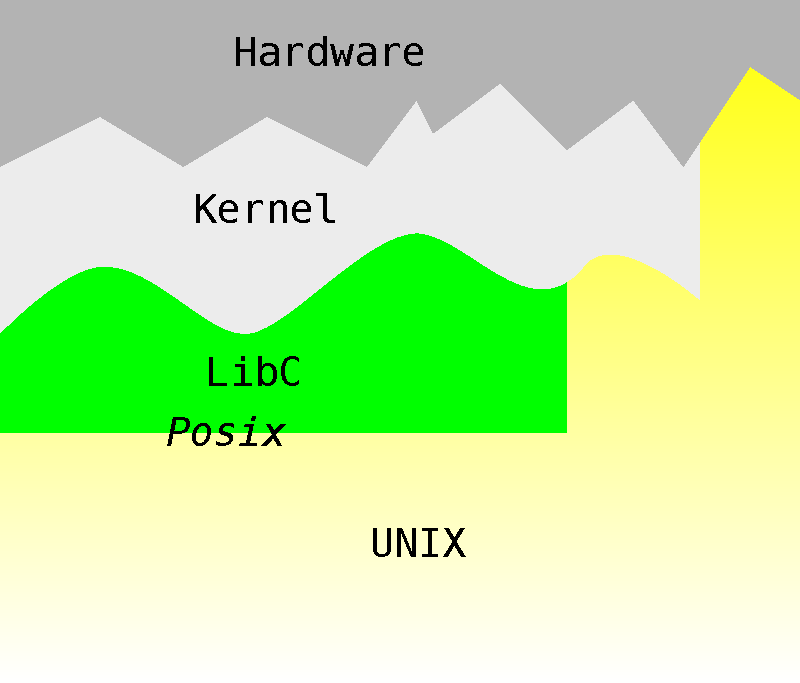
\includegraphics[width=8cm]{layers.pdf}
 \end{center}
\end{frame}

\begin{frame}{Die Komponenten}{für \target}
 \begin{description}
  \item[Hardware] \target
  \item[Kernel] zugeschnitten auf \target
  \begin{itemize}
    \item {\tiny \url{github.com/beagleboard/linux}}
  \end{itemize}	
  \item[root] das Filesystem
  \begin{description}
   \item[LibC] glibc 
   \begin{itemize}
    \item {\tiny \url{www.gnu.org/software/libc/index.html}}
   \end{itemize}	
   \item[\unix] busybox
   \begin{itemize}
    \item {\tiny \url{www.busybox.net/}}
   \end{itemize}
   \item[...] Weitere \unix basierte Komponenten
   \begin{itemize}
    \item das \cod{configure}, \cod{make}, \cod{make install} Triple 
   \end{itemize}
   \end{description}
 \end{description}
\end{frame}

\subsection{\host}
\begin{frame}{Toolchain}
 \begin{description}
  \item[binutils] linker \& Co.
  \item[gcc] compiler
  \begin{itemize}
   \item \cod{libgcc} die Bibliothek für den Compiler
  \end{itemize}
 \end{description}
 
 \begin{remarks}
 \item die Toolchain muss zweimal gebaut werden
 \begin{itemize}
  \item für den \kernel und \cod{libc} 
  \item für \unix/\posix
 \end{itemize}
 \item das target
 \begin{itemize} 
  \item \cod{cpu-vendor-os}
  
 \end{itemize}
 \end{remarks}
\end{frame}

\begin{frame}{Die Verzeichnisstruktur}
\dirtree{%
 .1 {\em somewhere\_on\_the\_host}.
 .2 tools.
 .3 config.sh \DTcomment{used in (all) scripts}.
 .3 {\em component}.sh \DTcomment{how to build}.
 .2 build \DTcomment{home of the build files}.
 .3 {\em component} \DTcomment{directory}.
 .2 target-root \DTcomment{top of targer root}.
 .2 tc \DTcomment{the new toolchain}.
 .2 config \DTcomment{of some components}.
 .2 mount \DTcomment{for mounting the \targetS (sshfs)}.
}
\end{frame}


%-------------------------
%minimal-unix
%(c) H.Buchmann FHNW 2014
%export TEXINPUTS=${HOME}/fhnw/edu/:${HOME}/fhnw/edu/tinL/config/latex:${HOME}/fhnw/edu/config//:
%-------------------------
\setlength{\TPHorizModule}{1mm}
\setlength{\TPVertModule}{1mm}

\newcommand{\qemu}{{\em qemu}\xspace}
\newcommand{\busybox}{{\em busybox}\xspace}
\newcommand{\yocto}{{\em yocto}\xspace}

\section{Toolchain}
\begin{frame}{Toolchain}{tc}
 \begin{itemize}
  \item die grossen zwei:
  \begin{itemize}
  \item Compiler
  \item Linker
  \end{itemize}
  \item kleinere Programme:
  \begin{itemize}
   \item Assembler
   \item ...
  \end{itemize}
 \end{itemize}
\end{frame}

\begin{frame}{Toolchain}{Beispiel}
 \begin{itemize}
  \item Sourcefile \cod{\{c|cc\}-source.\{c|cc\}}
  \item Compilat/object File \cod{\{c|cc\}-source.o}
  \item Executable/Image \cod{\{c|cc\}-source}
 \end{itemize}
\end{frame}

\subsection{Cross toolchain}
\begin{frame}{Cross toolchain}{2 Verschiedene Rechner}
\begin{description}[Cross\{Programm\}]
 \item[Host] Workstation leistungsfähiger Rechner
 \item[Target] Eingebettetes System (\beaglebone)
 \item[Cross\{Programm\}] Programm (Compiler etc.) das
 \begin{itemize}
  \item läuft auf dem {\em Host} und erzeugt Files für das {\em Target}
 \end{itemize}
\end{description}
\end{frame}

\begin{frame}{Cross toolchain}
 \begin{itemize}
  \item erzeugt auf dem {\em Host} Programme für das {\em Target}
 \end{itemize}
\end{frame}

\subsection{GNU/Toolchain}

\begin{frame}{GNU/Toolchain}{Zwei Komponenten}
\begin{description}[binutils]
 \item[binutils] Linker, assembler, ...
 \item[gcc] Compiler
\end{description}
\end{frame}

\subsection{Das klassische Build}
\begin{frame}{Build}{die drei Schritte}
 \begin{itemize}
  \item configure
  \item make
  \item make install
 \end{itemize}
 \remark{auf dem {\Huge Host}}
\end{frame}

\begin{frame}{Build}{der Kontext}
 \begin{description}
  \item[prefix] wo die Toolchain auf dem {\em Host} installiert wird
  \begin{itemize}
   \item option \cod{--prefix={\em path-to-toolchain-install}} 
  \end{itemize}
  \item[sysroot] wo ist das {\em Target} root system (auf dem {\em Host})
  \begin{itemize}
   \item option \cod{--with-sysroot={\em path-to-target-sysroot}}
  \end{itemize}
  \item[target] was für eine {\em Target} System
  \begin{itemize}
   \item option \cod{--target=armv6l-unknown-linux-gnueabihf}
   \remark{Warum ???}
  \end{itemize}
 \end{description}
\end{frame}


\section{Build}
\begin{frame}{Prinzip}
 \begin{itemize}
  \item wir sind in \cod{17-build}
  \item pro Komponente ein Skript in \cod{tools}
  \item pro Komponente ein Unterverzeichnis in \cod{build}
  \item der File \cod{tools/common.sh}
  \begin{itemize}
   \item Pfadnamem
  \end{itemize}
 \end{itemize}
\end{frame}

\subsection{Initiales \linux}
\begin{frame}{Build 1}{Toolchain 1}
 \begin{itemize}
  \item \cod{binutils.sh}
  \item \cod{gcc-bare.sh} 
  \begin{itemize}
   \item nur f�r den {\em kernel}
   \item das bare minimum
   \item nur {\Large C}
  \end{itemize}
 \end{itemize}
\end{frame}

\begin{frame}{Build 2}{Kernel}
 \begin{itemize} 
  \item \cod{kernel.sh} mit ein paar {\em targets}
   \begin{itemize}
    \item \cod{bb.org\_defconfig}
    \item \cod{zImage}
    \item \cod{headers\_install} 
	\begin{itemize}
	 \item Interface: {\em kernel}-{\em libc}
	\end{itemize}
   \end{itemize}
  \end{itemize}
\end{frame}

\begin{frame}{Build 3}{libc}{Wir brauchen glibc}
 \begin{itemize} 
  \item \cod{glibc} 
 \end{itemize}
\end{frame}

\begin{frame}{Build 4}{Toolchain 2}
 \begin{itemize} 
  \item \cod{gcc.sh} 
  \begin{itemize}
   \item mit \cod{sysroot}
   \item {\Large C} und {\Large C++}
  \end{itemize}
  \item Test
  \begin{itemize}\item im Verzeichnis \cod{work}\end{itemize}
 \end{itemize}
\end{frame}

\begin{frame}{Build 5}{busybox}
 \begin{itemize}
  \item \cod{busybox.sh}
  \begin{itemize}
   \item Installation auf SD-Card
   \item \cod{fakeroot}
  \end{itemize}
 \end{itemize}
\end{frame}


\begin{frame}{Skripts und Argumente}{initiales System}
 \begin{tabular}{l|l|l}
  Skript & target & gebraucht f�r\\
  \hline\hline
  \cod{binutils.sh}& &alles\\
  \hline
  \cod{gcc-bare.sh}& &kernel, libc\\
  \hline
  \cod{kernel.sh}  & \cod{defconfig}\\
                   & \cod{zImage}\\
                   & \cod{headers\_install}\\
  \hline
  \cod{glibc.sh}  & &POSIX\\
  \hline
  \cod{gcc.sh}     & &C/C++, POSIX\\
  \hline
  \cod{busybox.sh} & \cod{busybox}\\
  		   &\cod{install}\\
  \hline
  \cod{target-root.sh}&&Transfer auf SD-Card
 \end{tabular}
 \remark{Alle Skripte sind {\Large\tt bash} Skripte}
\end{frame}

\begin{frame}{Target}{erster Versuch}
\begin{itemize}
 \item transfer auf SD Karte
 \item Internet
\end{itemize}
\end{frame}

\begin{frame}{Skripts und Argumente}{ssh}
\begin{tabular}{lll}
 \cod{zlib.sh}\\
 \cod{openssl.sh}&&die kryptographischen Algorithmen\\
 \cod{openssh.sh}
\end{tabular}
\remark{\cod{openssh.sh} h�ngt von \cod{zlib.sh} und \cod{openssl.sh}
  ab}
\end{frame}

\subsection{ssh}
\begin{frame}{\cod{ssh}}
 \begin{itemize}
  \item \cod{openssh} die volle Implementation 
  \begin{itemize}
   \item \cod{zlib}
   \item \cod{openssl}
   \item \cod{openssh}
  \end{itemize}
%  \item \cod{sshfs}
 \end{itemize}
\end{frame}

\subsection{Workflow}
\begin{frame}{Workflow}{Begriffe}
\begin{description}[target-root]
 \item[target-root] Verzeichnis auf dem \host
 \begin{itemize}
  \item enth�lt das \target Rootfilesystem
  \item soll aktuell sein
 \end{itemize}
 \item[SD-Card] Speicherkarte mit dem \target Rootfilesystem
 \begin{itemize}
  \item entspricht  \cod{target-root}
 \end{itemize}
\end{description}
\end{frame}

\begin{frame}{target-root - SD-Card}{\cod{tar} \cod{rsync}}

\begin{tabular}{lcccc}
	&target-root&&SD-Card\\
\hline	
initiales \linux &$\to$& \cod{tar}   &$\to$\\
SD-Card          &$\leftarrow$& \cod{rsync} &$\leftarrow$\\  
target-root      &$\to$& \cod{rsync} &$\to$
\end{tabular}
\end{frame}

%\begin{frame}{Target}{ssh}
%\begin{itemize}
% \item \cod{ssh}
% \item \cod{sshd}
% \item Keys
%\end{itemize}
%\end{frame}

\begin{frame}{sshfs}{funktioniert noch nicht}
 \begin{itemize}
  \item Die Bibliothek \cod{glib}
  \item Ersatz
  \begin{itemize}
   \item \cod{sftp}
  \end{itemize}
 \end{itemize}
\end{frame}



\section{Configure}
\begin{frame}{{\em configure}-{\em make}-{\em make install}}{Installation neuer Komponenten}
 \begin{itemize}
  \item aus den Quellen
  \item immer etwa gleich
  \begin{itemize}
   \item download
   \item \cod{configure {\em options}}
   \item \cod{make}
   \item \cod{make install}
  \end{itemize}
  \item Unterschiede in den Details
 \end{itemize}
\end{frame}

\begin{frame}{\url{rsync.samba.org}}{als Beispiel}
 \begin{itemize}
  \item auf dem \host
  \item auf dem \targetS
 \end{itemize}
\end{frame}


\subsection{Auf dem \host}

\begin{frame}{Verzeichnisstruktur}
 \begin{itemize}
  \item Source:\cod{rsync-3.1.2}
  \item Build:   für die (vielen) Zwischenfiles
  \item Install: prefix
  \item rsync.sh: das Skript
 \end{itemize}
\end{frame}

\begin{frame}{Skript: \cod{rsync.sh}}{schrittweise für den \host}
 \begin{itemize}
  \item \cod{configure --help}
  \item \cod{configure --prefix}
  \begin{itemize}
   \item prefix: wohin kommt das Resultat
   \item Files in \cod{rsync-build}
  \end{itemize}
  \item \cod{make}
  \begin{itemize}
   \item Files in \cod{rsync-build}
  \end{itemize}
  \item \cod{make install}
  \begin{itemize}
   \item Files in \cod{prefix}
  \end{itemize}
 \end{itemize}
\end{frame}

\begin{frame}{Aufgabe Skript: \cod{rsync.sh}}{für \targetS}
 \begin{itemize}
  \item Crosscompile \cod{--sysroot}
  \item \cod{--prefix}
  \item \cod{DESTDIR}
 \end{itemize}
 \remark{tools/rsync.sh}
\end{frame}


\part{Build again}
\frame{\titlepage}
\frame{\partpage}
\begin{frame}{Basics}
 \begin{itemize}
  \item Toolchain: 
  \begin{itemize}
   \item bare
  \end{itemize}
  \item Kernel:
  \begin{itemize}
   \item ohne module
   \item ohne unötigen {\em drivers}
   \item USB Gadgets
  \end{itemize}
  \item libc:
  \begin{itemize}
   \item glibc
  \end{itemize}
  \item Toolchain: 
  \begin{itemize}
   \item voll inkl C++
  \end{itemize}
  \item busybox:
 \end{itemize}
\end{frame}

\begin{frame}{Supplement}{Internet}
 \begin{itemize}
  \item ssh
  \begin{itemize}
   \item zlib
   \item openssl
   \item openssh
  \end{itemize}
  \item init
  \begin{itemize}
   \item usb - ethernet
   \item ssh
   \item {\Large neu} \cod{ntp}
   \begin{itemize}
    \item network time protocol
   \end{itemize}
  \end{itemize}
 \end{itemize}
\end{frame}

\begin{frame}{Supplement}{Wi-Fi}
 \begin{itemize}
  \item wpa\_supplicant
  \begin{itemize}
   \item Configuration
  \end{itemize}
 \end{itemize}
\end{frame}

\begin{frame}{Noch nicht gut gelöst}
 \begin{itemize}
  \item die Verbindung {\bf RootFS}
  \begin{itemize}
   \item \host $\leftrightarrow$ \targetS
  \end{itemize}
  \item Versionen
  \begin{itemize}
   \item wie ist ein RootFS erzeugt worden
  \end{itemize}
 \end{itemize}
\end{frame}


%\section{Modules}
%\begin{frame}{Modules}
%\begin{itemize}
% \item siehe \cod{6-modules}
%\end{itemize}
%\end{frame}
%
%\begin{frame}{Modules}{Verzeichnisstruktur}
%\begin{block}{Host}
%\dirtree{%
% .1 BUILD\_HOME.
% .2 modules.
% .3 Makefile \DTcomment{for own modules}.
% .3 *.{c/h} \DTcomment{the own sources}.
% .2 scripts.
% .3 module.sh.
%}
%\end{block}
%\begin{block}{\target}
%\dirtree{%
%.1 /.
%.2 work.
%}
%\end{block}
%\end{frame}
%\begin{frame}{Herstellung}{Workflow}
% \begin{block}{Host}
% \begin{itemize}
%  \item \cod{sh scripts/module.sh {\em module}}
%  \item \cod{scp}, \cod{sftp}, \cod{ftp}
% \end{itemize}
% \end{block}
% \begin{block}{\target}
%  \begin{itemize}
%   \item \cod{insmod}
%   \item \cod{rmmod}
%  \end{itemize}
% \end{block}
%\end{frame}

%\part{Installation TFT Display}
%\section{Installation TFT Display}
\frame{\partpage}
\begin{frame}{Um was geht es ?}{Adafruit TFT Touchscreen}
 \begin{itemize}
  \item Installation auf einem minimalen System
  \item \cod{git} update
  \item Konfiguration
  \item Kernelcompilation
  \item Driver
  \item Module
  \item {\em framebuffer}
 \end{itemize}
\end{frame}

\begin{frame}{Hardware}
 \begin{itemize}
  \item {\tiny\url{https://learn.adafruit.com/adafruit-2-8-pitft-capacitive-touch/downloads}}
  \item Zwei Chips
  \begin{itemize}
   \item \cod{STMPE610} für den {\em touchscreen}
   \item \cod{ILI9341} für die Graphik
  \end{itemize}
  \item Verbunden per \cod{SPI}
  \end{itemize}
\end{frame}

\begin{frame}{Funktionierendes System}
\begin{itemize}
 \item {\tiny \url{http://adafruit-download.s3.amazonaws.com/2015-02-16-raspbian-pitft28r_150312.zip}}
 \item Verbindung per \cod{ssh}
 \begin{remarks}
  \item user \cod{pi}
  \item pw: \cod{raspberry}
 \end{remarks}
 \item Host \cod{dhcp}
 \item Host \cod{nmap}
 \item Framebuffer \cod{/dev/fb*}
 \begin{itemize}
  \item alles ist ein File
 \end{itemize}
 \item Backlight Control
\end{itemize}
\end{frame}

\begin{frame}{Kernel}{Neue Version}
\begin{itemize}
 \item \cod{git pull}
 \item \cod{drivers/staging/fbtft/fb\_ili9341.c}
\end{itemize}
\end{frame}

\section{Module}

\begin{frame}{Module herstellen}
 \begin{itemize}
  \item als Modul herstellen: {\em menuconfig}
  \begin{itemize}
   \item \cod{FB\_TFT\_FBTFT\_DEVICE}
   \begin{itemize}\item\cod{drivers/staging/fbtft/fbtft\_device.c}\end{itemize}
   \item \cod{FB\_TFT\_ILI9341}
   \begin{itemize}\item\cod{drivers/staging/fbtft/fb\_ili9341.c}\end{itemize}
  \end{itemize}
  \item nur einzelne Module herstellen
  \begin{itemize}
   \item {\em dir/file.ko}
   \begin{itemize}
    \item {\em dir} relativ zu kernel source
   \end{itemize}
  \end{itemize}
 \end{itemize}
\end{frame}

\begin{frame}{Module ausführen}
 \begin{itemize}
  \item zum {\em target} kopieren
  \item \cod{insmod {\em name parameters}}
  \item \cod{mkdev -s} erzeugt \cod{/dev/fb1}
  \item siehe auch
   \begin{itemize}\item\cod{/sys/class/graphics/}\end{itemize}
 \end{itemize}
\end{frame}

\begin{frame}{Zusätzliche Infos}{von einem funktionierenden System}
 \begin{itemize}
  \item \cod{dmesg-wheezy-raspbian.log}
  \ite \cod{config-wheezy-raspbian.gz}
 \end{itemize}
\end{frame}

\end{document}
